\documentclass[fleqn,10pt]{olplainarticle}
\usepackage{float}
\usepackage{tikz}
\usepackage{caption}
\usepackage{subcaption}
\usepackage{hyperref}
\hypersetup{
    colorlinks=false,
    pdfborder={0 0 0},
}

% Use option lineno for line numbers 
\title{What is the cause and effect in ship data analysis, when all we can see is correlation?}

\author[1,2]{Martin Alexandersson}
\affil[1]{Research Institutes of Sweden (RISE), Chalmers tvärgata 10, 41296 Gothenburg Sweden}
\affil[2]{Dept. of Mechanics and Maritime Sciences, Division of Marine Technology,
                                Chalmers University of Technology, Hörsalsvägen 7A, Gothenburg Sweden}

\keywords{Ship dynamics, Causal inference, System identification, Monte Carlo simulations, Markov chain analysis}



\begin{abstract}
%Purpose and scope

%Methods

%Results

%Conclusion
\end{abstract}

\begin{document}
\def\equationautorefname~#1\null{Eq.~(#1)\null}
\def\figureautorefname~#1\null{Figure~#1\null}
\def\tableautorefname~#1\null{Table~#1\null}

\flushbottom
\maketitle
\thispagestyle{empty}
\newpage
\section{Introduction}
%________________________________________
%Situation:
As humans, we often think in terms of cause and effect (causality) — if we understand why something happened, we can change our behavior to improve future outcomes. The same goes for ships, if we understand how they work, we can operate them in safer and more energy efficient ways. 
Causal inference is a process of determining the causality. Conducting experiments is a way to infer causality where the effect of one variable can be studied in isolation. Such experiments can be conducted for ships using scale models tested in a controlled laboratory environment.
The use of scale models may introduce problems with scale effects. The laboratory environment as well as the test scenario being artificial idealizations of their real counterparts is also problematic. 

Data driven analysis on real ship operational avoids these problems and is a more relevant way to analyze the ship's operation. Causal inference is however much harder when using operational data, since that data was not collected from a controlled experiment. The data analysis can show how variables vary together (correlation). The correlation does not imply direct causality where \emph{A} causes \emph{B} (\autoref{fig:direct_causation}). \emph{A} and \emph{B} could also have the opposite relation in reversed causality (\autoref{fig:reversed_causation}) for example:
\begin{quote}
\emph{Do windmills generate the wind, or is it the other way around?}
\end{quote}
\emph{A} and \emph{B} can also be caused by a third hidden variable \emph{C} (common causality) (\autoref{fig:common_causation}), for instance:
\begin{quote}
\emph{If ice cream sales increase, the rate of drowning deaths also increases, so should you avoid ice cream when swimming?}
\end{quote}
\begin{figure}[!htb]
    \begin{subfigure}[b]{0.3\textwidth}
        \centering
        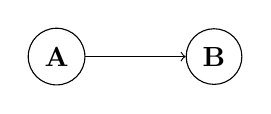
\begin{tikzpicture}[node distance=2cm]
        \node[circle,draw] at (0,0) (A) {\bf A};
        \node[circle,draw,right of=A] (B) {\bf B};
        \draw[->] (A) -- (B);
        \end{tikzpicture}
        \caption{Direct causality}
        \label{fig:direct_causation}
    \end{subfigure}
    \hfill
    \begin{subfigure}[b]{0.3\textwidth}
        \centering
        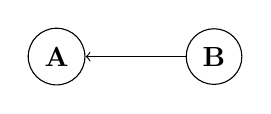
\begin{tikzpicture}[node distance=2cm]
        \node[circle,draw] at (0,0) (A) {\bf A};
        \node[circle,draw,right of=A] (B) {\bf B};
        \draw[<-] (A) -- (B);
        \end{tikzpicture}
        \caption{Reversed causality}
        \label{fig:reversed_causation}
    \end{subfigure}
    \hfill
    \begin{subfigure}[b]{0.3\textwidth}
        \centering
        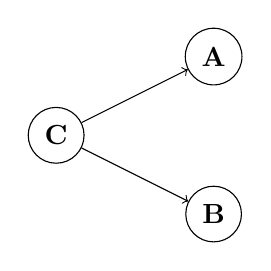
\begin{tikzpicture}[node distance=2cm]
        \node[circle,draw] at (0,0) (C) {\bf C};
        \node[circle,draw,right of=C,yshift=1cm] (A) {\bf A};
        \node[circle,draw,right of=C,yshift=-1cm] (B) {\bf B};
        \draw[->] (C) -- (A);
        \draw[->] (C) -- (B);
        \end{tikzpicture}
        \caption{Common causality}
        \label{fig:common_causation}
    \end{subfigure}
    \caption{Causality}
    \label{fig:causal_relationships}
    
\end{figure}
%\subsection{Case study}
Determining the causality from real world data is a difficult but important task. For instance proving that the emission of green house gases causes global warming is perhaps the most important task of our time? A more modest task is addressed in this paper; The thruster balance of a double ended ferry Uraniborg (\autoref{fig:uraniborg}) is to be optimized for fuel consumption reduction. 
\begin{figure}[!htb]
    \centering
    \includegraphics[width=0.7\textwidth]{figures/GA_uraniborg.pdf}
    \caption{Double ended ferry Uraniborg, copyright Rederi AB Ventrafiken.}
    \label{fig:uraniborg}
\end{figure}

The propulsion arrangement of Uraniborg consists of two azimuth thrusters, one in the aft and one in the forward part of the ship (\autoref{fig:uraniborg}). The two thrusters can run simultaneously adding up to the total thrust force that drives the ship forward. The load balance between the thrusters can vary from full forward or aft thruster utilization, to a 50-50\% split between the thrusters. With the aim of load balance optimization, operational data collected onboard Uraniborg has previously been analyzed. The load balance was measured as a coefficient ($r_{aft}$) representing the utilization of the aft thruster as defined in \autoref{eq:aft_thrust_ratio},
\begin{equation}
    r_{aft} = \frac{C_{aft}}{C_{aft} + C_{fwd}}
    \label{eq:aft_thrust_ratio}
\end{equation}
where $C_{aft}$ and $C_{fwd}$ are the fuel consumption from the aft and forward thruster.
High correlation between $r_{aft}$ and total fuel consumption was observed for trips during one year with Uraniborg between Landskrona and the island of Ven as seen in \autoref{fig:fuel_consumption_correlation}.
\begin{figure}[!htb]
    \centering
    \includegraphics[width=\textwidth]{figures/correlation.pdf}
    \caption{Fuel consumption per trip with Uraniborg for trips during one year with varying aft thrust ratio.}
    \label{fig:fuel_consumption_correlation}
\end{figure}

%________________________________________
%Problem:
The correlation implies that there is a relationship between $r_{aft}$ and the fuel consumption; However, it is not possible to conclude which kind of causality (\autoref{fig:causal_relationships}). A direct causality that higher aft thruster utilization ($r_{aft}$) reduces the fuel consumption, would be very useful to optimize the fuel consumption. However, both reversed causality or common causality are also possibilities, considering other hypothetical scenarios:
\begin{itemize}
    \item Increased fuel consumption forces a reduced aft thruster utilization if the aft thruster is not strong enough. The forward thruster is then needed to add up to the higher power demand. (Reversed causality)
    
    \item There is a hidden variable such as bad weather which forces both thrusters to be used. (Common causality)
\end{itemize}
%________________________________________
%Solution:
The causal inference for the aft thruster utilization is presented in this paper by conducting a blinded experiment onboard Uraniborg. Alternative ways for causal inference are also presented; The alternatives are intended to be used when experiments are not possible, or very inconvenient to conduct.

%________________________________________
%Evaluation:
The result from the experiment is analyzed to infer the direct causality between the aft thruster utilization and the fuel consumption. It is also investigated if alternative causal inferences can arrive to the same conclusion.  

\section{Method}
A blinded experiment (\autoref{sec:blinded_experiment}) is the classic way to determine the causation. For situations where experiments cannot be conducted system identification with well established
mathematical models, Monte Carlo simulations and Markov chain analysis are other methods.

\subsection{Blinded experiment}\label{sec:blinded_experiment}
In the blinded experiment, every other trip with Uraniborg was run with two different crews. One crew was operating as normal and the other crew was instructed to only use the aft thruster as much as possible. The same correlation that was seen in \autoref{fig:fuel_consumption_correlation} was observed again during the experiment and a direct causation was concluded that a higher use of the aft thruster will reduce the fuel consumption.

\subsection{System identification}
\subsection{Monte Carlo simulations}
\subsection{Markov chain analysis}

\bibliography{sample}

\end{document}